\documentclass{article}

\usepackage{array}
\usepackage{graphicx}

\begin{document}

\title{Week 9, Day 1 Problems}
\author{GSI: Caleb Eades}
\date{10/16}
\maketitle

\section{Potential Midterm Potentials}

\subsection{Conductors}

An uncharged solid conducting sphere of radius $R$, centered at the origin, contains two spherical cavities or radii $r_1$ and $r_2$, respectively. Point charge $Q_1$ is then placed within the cavity of radius $r_1$, and point charge $Q_2$ is then placed within the cavity of radius $r_2$, as shown below. Determine the resulting electric field vector for $r>R$, where $r$ is the distance from the origin.

(\textit{Source: Birgeneau Fall 2015 Midterm 2, Problem 2})

\begin{figure}[h]
	\begin{center}
	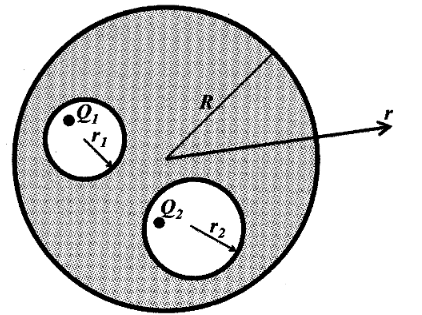
\includegraphics[width=0.5\textwidth]{ConductorMid.png}
	\end{center}
\end{figure}

\subsection{Rods}

Consider a thin rod of length $2d$ centered on the $x$-axis as shown. The rod has a non-uniform linear charge distribution $\lambda=ax$. Determine the potential $V$ for
\begin{itemize}
	\item[(a)] a point along the $y$-axis at a distance $y_0$ from the origin
	\item[(b)] points along the $x$-axis outside the rod, at a distance $x_0$ from the origin
\end{itemize}

(\textit{Source: Birgeneau Fall 2015 Midterm 2, Problem 3})

\begin{figure}[h]
	\begin{center}
	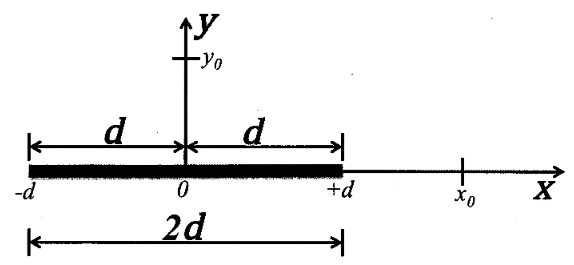
\includegraphics[width=0.5\textwidth]{RodMid.png}
	\end{center}
\end{figure}

\subsection{Connected Conductors}

Two conducting globes (spherical shells) with radii $r_1$ and $r_2$, with $r_2=2r_1$, are joined by a long thin wire. +ve charge is steadily added to the system until a faint glow is seen around one of the spheres, a consequence of ionisation of the air nearby. Which is it? (no credit for simply giving the answer without proof).

(\textit{Source: Bloxham Summer 2015 Midterm 2, Problem 2})

\subsection{The Slab}

The figure shows an infinite slab of charge that has a width, $d$, and within which the charge density, $\rho(x)=\rho_0cos\left(\frac{n\pi x}{d}\right)$.
\begin{itemize}
	\item[(a)] The electric field is zero for $x\leq0$ \textbf{and} $x\geq d$. What, then, are the possible values of $n$?
	\item[(b)] Take $V(0)=0$. Under the conditions in part a, what is the electric potential, $V(x)$, inside the slab (for $0\leq x\leq d$)? Express it in terms of $n$, $\pi$, $\rho_0$, $\epsilon_0$, $d$, and $x$.
\end{itemize}

(\textit{Source: Speliotopoulos Spring 2014 Midterm 2, Problem 2})

\begin{figure}[h]
	\begin{center}
	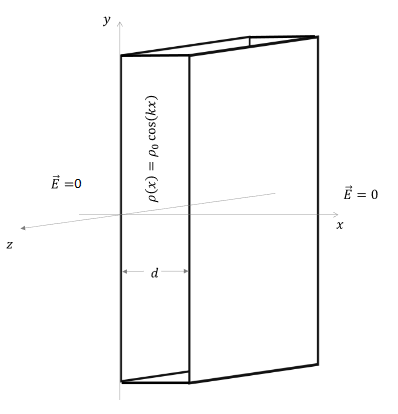
\includegraphics[width=0.5\textwidth]{SlabMid.png}
	\end{center}
\end{figure}

\end{document}
